%%%%%%%%%%%%%%%%%%%%%%%%%%%%%%%%%%%%%%%%%%%%%%%%%%%%%%%%%%%%%%%%%%%%%%%%%%%
\chapter{Include JSXGraph into web pages}\label{ch:start}

\section{Additional files}
For including JSXGraph into HTML, two files are necessary:
\begin{itemize}
    \item jsxgraphcore.js
    \item jsxgraph.css
\end{itemize}
You can either download these two files and use the local copy or you can use the online version.
Then, the beginning of the HTML file should start like this:
\begin{fullwidth}\begin{lstlisting}[language=HTML]
<html>
<head>
 <link rel="stylesheet" type="text/css" href="jsxgraph.css" />
 <script type="text/javascript" src="jsxgraphcore.js"></script>
</head>
<body>
...
</body>
</html>
\end{lstlisting}\end{fullwidth}
If you want to include the online version of JSXGraph in your HTML file then you have to write the following lines into the document head:
\begin{fullwidth}\begin{lstlisting}[language=HTML]
<html>
<head>
 <link rel="stylesheet" type="text/css" 
  href="http://jsxgraph.uni-bayreuth.de/distrib/jsxgraph.css" />
 <script type="text/javascript" 
  src="http://jsxgraph.uni-bayreuth.de/distrib/jsxgraphcore.js"></script>
</head>
<body>
...
</body>
</html>
\end{lstlisting}\end{fullwidth}

\section{The drawing panel}

The geometric construction which is displayed by JSXGraph resides in an HTML element. Usually, a div-element is taken. This division needs a unique ID. This ID will connect the HTML element with our JavaScript code.

The following code has to be placed into the body part of an HTML file:
\begin{fullwidth}\begin{lstlisting}[language=HTML]
<div id="box" class="jxgbox"  style="width:500px; height:500px;"></div>
<script type="text/javascript"> 
 var board = JXG.JSXGraph.initBoard('box', {boundingbox:[-5,5,5,-5], axis:true});
</script>
\end{lstlisting}\end{fullwidth}
The division gets the ID 'box'. The JSXGraph board is initialized with the method
\lstinline|JXG.JSXGraph.initBoard()|. \lstinline|JXG| is a global object defined in jsxgraphcore.js. All JSXGraph objects
are subobject of \lstinline|JXG|, i.e. it defines the JSXGraph namespace.

We can use as many different drawing panels as we like in one HTML file. The class jxgbox sets the CSS property ``position:relative'' which seems to be mandatory for the Internet Explorer 7. 

Then, the web browser should display an element like the one shown in Figure~\ref{fig:1}.
\begin{figure*}[htb]
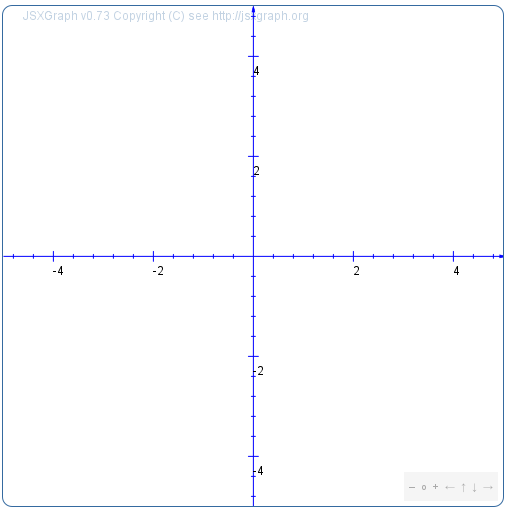
\includegraphics[width=0.4\linewidth]{images/b2.png}
\caption{The first JSXGraph construction.}\label{fig:1}
\end{figure*}

\noindent
The complete HTML file then looks like this:
\begin{fullwidth}\begin{lstlisting}[language=HTML]
<html>
<head>
 <link rel="stylesheet" type="text/css" href="jsxgraph.css" />
 <script type="text/javascript" src="jsxgraphcore.js"></script>
</head>
<body>
<div id="box" class="jxgbox" style="width:500px; height:500px;"></div>
<script type="text/javascript">
 var board = JXG.JSXGraph.initBoard('box', {boundingbox:[-5,5,5,-5], axis:true});
</script>
</body>
</html>
\end{lstlisting}\end{fullwidth}

\noindent
The method \lstinline|initBoard()| has two parameters: the first parameter is the ID of the HTML element
that will contain our construction, e.g. 'box'. The second, optional parameter is a JavaScript object -- enclosed
in curly brackets \lstinline|{}| -- containing options to control the display of the board. These options are
separated by kommas.
The possible optional properties of the board are:
\begin{itemize}
    \item boundingbox
    \item axis (true/false)
    \item grid (true/false)
    \item showNavigation (true/false)
    \item showCopyright (true/false) 
    \item zoomX, zoomY
    \item originX, originY (in pixel)
    \item unitX, unitY (in pixel)
\end{itemize}
